\documentclass[12pt]{article}
\usepackage{geometry}
\geometry{left=1in,right=0.75in,top=1in,bottom=1in}
\newcommand{\Problem}{E}
\newcommand{\Team}{2523245}
\usepackage{newtxtext}
\usepackage{amsmath,amssymb,amsthm}
\usepackage{newtxmath} % must come after amsXXX
\usepackage[pdftex]{graphicx}
\usepackage{xcolor}
\usepackage{fancyhdr}
\usepackage{booktabs}
\usepackage{changepage}
\usepackage{enumitem}
\usepackage{subcaption}
\usepackage{makecell}
\usepackage{multirow}
\usepackage{algorithm}
\usepackage{caption}
\usepackage{algpseudocode}
\captionsetup{skip=0.05cm}
\lhead{Team \Team}
\rhead{}
\cfoot{}
\newtheorem{theorem}{Theorem}
\newtheorem{corollary}[theorem]{Corollary}
\newtheorem{lemma}[theorem]{Lemma}
\newtheorem{definition}{Definition}
\begin{document}
	\graphicspath{{.}}  % Place your graphic files in the same directory as your main document
	\DeclareGraphicsExtensions{.pdf, .jpg, .tif, .png}
	\thispagestyle{empty}
	\vspace*{-16ex}
	\centerline{\begin{tabular}{*3{c}}
			\parbox[t]{0.3\linewidth}{\begin{center}\textbf{Problem Chosen}\\ \Large \textcolor{red}{\Problem}\end{center}}
			& \parbox[t]{0.3\linewidth}{\begin{center}\textbf{2025\\ ICM\\ Summary Sheet}\end{center}}
			& \parbox[t]{0.3\linewidth}{\begin{center}\textbf{Team Control Number}\\ \Large \textcolor{red}{\Team}\end{center}}	\\
			\hline
	\end{tabular}}
	%%%%%%%%%%%%%%% 环境配置结束 %%%%%%%%
	%%%%%%%%%%% Summary开始 %%%%%%%%%%%
	\setcounter{page}{1}
	\begin{center}
		\Large{\textbf{Title Here.}}
		\vspace{0.2cm}
		
		
		
		
		\large{\textbf{Summary}}
		\vspace{-0.4cm}
	\end{center}
	Summary begins here..
	
	%%%%%%%%%%% Summary结束 %%%%%%%%%%%
	%%%%%%%%%%%% 生成目录 %%%%%%%%%%%%
	\clearpage
	\pagestyle{fancy}
	\tableofcontents 
	\newpage
	\rhead{Page \thepage\ }
	%%%%%%%%%%% 生成目录结束 %%%%%%%%%%%%%
	%%%%%%%%%% 正文开始 %%%%%%%%%%%%%%
	\section{Introduction}
	\section{Assumption and Justification}
	\section{Notations}
	
	\begin{table}[h]
		\centering
		\begin{tabular}{cc}
			\toprule[2pt]
			\textbf{Notations} & \textbf{Explanations} \\
			\midrule[1pt]
			$RTS$ & Resistance Stability \\
			$RLS$ & Resilience Stability \\
			$TES$ & Total Ecosystem Stability \\
			\bottomrule[2pt]
		\end{tabular}
		\caption{notations}
		\label{notations}
	\end{table}
	\section{Food Web Model}
	$Food Web Model = Basic Food Web Model - Invasion Model$
	\subsection{Elementary Ecology Interaction Model, EEIM}
	\subsubsection{Food Web Dynamics}
	\hspace{2em}Food web dynamics serves to describe trends of interactions among species and the energy flow in ecosystem. Absorbing energies from the circumstances, producers pass them to consumers. Then via the metabolism of consumers and role of decomposers, the energies returned to external surroundings. On account of that the forest was newly converted to agricultural use, the chief species, including crops, insects and birds, their biomass is bound to change.We can apply Food Web Dynamics to research the process.
	
	On the premise of $n$ species, the dynamics of the community can be described by multiple differential equations:
	\begin{equation}
		\frac{dB_i}{dt}=f_i(B)\hspace{1em}(i=1,2,...,n)
		\label{Bi}
	\end{equation}
	where $Bi$ is the biomass of species $i$, $B$ is the vector for all species within the community.\\
	
	\subsubsection{Intra-Interspecific Interactions Among Species}
	\hspace{2em}For simplicity, we only focus on intraspecific interactions and feeding relationship in the area, of which intraspecific interactions depends on only the environment and the biomass of the population itself while feeding relationship is additionally influenced by the species with which it interacts. The latter can be referred to as Consumer-Resource(C-R) interactions[].Therefore, \ref{Bi} can be improved as:
	\begin{equation}
		\frac{dB_i}{dt}=f_i(B_i)+\sum_{j=1,j\neq i}^n f_{ij}(B_i,B_j)-\sum_{k=1,k\neq i}^n f_{ki}(B_i,B_k)\hspace{1em}(i=1,2,...,n)
	\end{equation}
	where $f_i(B_i)$ is intraspecific interaction term for species $i$, $f_{ij}(B_i,B_j)$ is resource contributions to $i$, and $f_{ik}(B_i,B_k)$ is loss caused by predator $k$.
	
	\textbf{As for producers},according to people's demands in agricultural ecosystem, we classify them into crops and weeds. During natural cycle, The increase of biomass relies on photosynthesis, the decrease is compose of interspecific competition, primary consumers' depletion and non-natural death. With respect to the chemical factors such as herbicides, we will analyze their effects in the Invasion Model later. Thus, the dynamic equation for producers can be expressed as:
	\begin{equation}
		\frac{dB_i}{dt}=r_iB_i(1-\frac{1}{K}\sum_{pro}B_k)-a_{ins-i}B_{insects}-d_iB_i
	\end{equation}
	where $r_i$ is intrinsic productivity of crops or weeds, $K$ is maximum carrying capacity for producers, $a_{ins-i}$ is interaction coefficient between crops or weeds and insects, $d_i$ is crops' or weeds' mortality.
	To better understand crop-weed competition, we modify \textbf{Logistic Equation} and get:
	\begin{equation}
		\begin{cases}
			\frac{dB_{crop}}{dt}=r_{crop}B_{crop}(1-\frac{B_{crop}}{K_{crop}}-\sigma_1\frac{B_{weed}}{K_{weed}})\\
			\frac{dB_{weed}}{dt}=r_{weed}B_{weed}(1-\frac{B_{weed}}{K_{weed}}-\sigma_2\frac{B_{crop}}{K_{crop}})
		\end{cases}
	\end{equation}
	
	\textbf{From the consumers' perspective}, we can derive \textbf{Lotka-Volterra  basic equation}:
	\begin{equation}
		\frac{dB_i}{dt}=B_i(b_i+\sum_{j=1,j\neq i}^n a_{ij}B_j)\hspace{1em}
	\end{equation}
	
	Insects, which are primary consumers, increase by digesting consumers and decrease due to being preyed upon and respiration.Their equation is:
	\begin{equation}
		\frac{dB_{insects}}{dt}=r_{insects}B_{insects}(1+a_{cro-ins}\frac{B_{crop}}{K_{crop}}+a_{wee-ins}\frac{B_{weed}}{K_{weed}}-a_{bir-ins}\frac{B_{bird}}{K_{bird}})
	\end{equation}
	where $x_{insects}$ is respiration rate of insects.
	
	Considering that in newly converted forest, the ecosystem is uncomplicated. Birds, as secondary consumers, have fewer predators so we can temporarily ignore the impacts of birds being preyed.Then, the birds' equation is:
	\begin{equation}
		\frac{dB_{bird}}{dt}=r_{bird}B_{bird}(1+a_{ins-bir}\frac{B_{insects}}{K_{insects}})
	\end{equation}
	
	The growth of \textbf{decomposers} owing to organic debris from producers, excreta from consumers and many other aspects, and they diminish due to predators and metabolism:
	\begin{equation}
		\frac{dB_{decomposers}}{dt}=a_{cro-de}B_{crop}+a_{wee-de}B_{wee}+a_{bir-de}B_{bir}-x_{decomposers}B_{decomposers}-\beta
	\end{equation}
	
	\subsubsection{Impacts of agricultural cycle and season}
	\hspace{2em}Given that ecosystems encompass both the biosphere and the natural environment,we explicitly incorporate the significant impacts of agricultural cycles and seasonal transitions on system dynamics.For this purpose, we select the region Q, situated within the temperate monsoon climate zone of the Northern Hemisphere, as the basis for our model development. In region Q,winter is characterized by cold and arid conditions, whereas summer is marked by high temperature and precipitation, with a cropping intensity allowing for two harvests per year. These climatic conditions exert a significant influence on the species diversity within the ecosystem, thereby necessitating their comprehensive consideration in our modeling framework to accurately depict the ecological dynamics.
	
	To quantify the combined effects of multiple factors on the ecosystem, we drew inspiration from the superposition principle in circuit analysis. We set the impacts of agricultural cycles and seasonal factors to zero to derive the relationship between population biomass and time. Then, we considered only the agricultural cycles and seasonal factors to obtain the relationship between biomass and time under these conditions. Finally, by summing these two relationships, we determined the comprehensive relationship between biomass and time.
	
	Considering only agricultural cycles and seasonal factors,we establish the function describing the variation of biomass over time as $P_x(t)$.
	\begin{equation}
		P_{x}(t)=P_{xmin}+k_{x}(P_{xmax}-P_{xmin})[1-A(t)]S(t)sin(\omega t+\phi)
	\end{equation}
	Then,we get the comprehensive biomass of each component in the ecosystem as $C_{x}(t)$.
	\begin{equation}
		C_{x}(t)=B_{x}(t)+P_{x}(t)
	\end{equation}
	where $x$ respectively represents "crop","weed","insects","birds"or"decomposers",$k$ refers to the degree of impact on different species, $A$ represents agricultural tillage intensity,$S$ is seasonal impact factor index.
	
	Eventually,the comprehensive biomass is calculated as follows.
	\begin{equation}
		C(t)=C_{producers}(t)+C_{consumers}(t)+C_{decomposers}(t)
	\end{equation}
	% 第一题的示波器
	\begin{figure}[t]
		\centering
		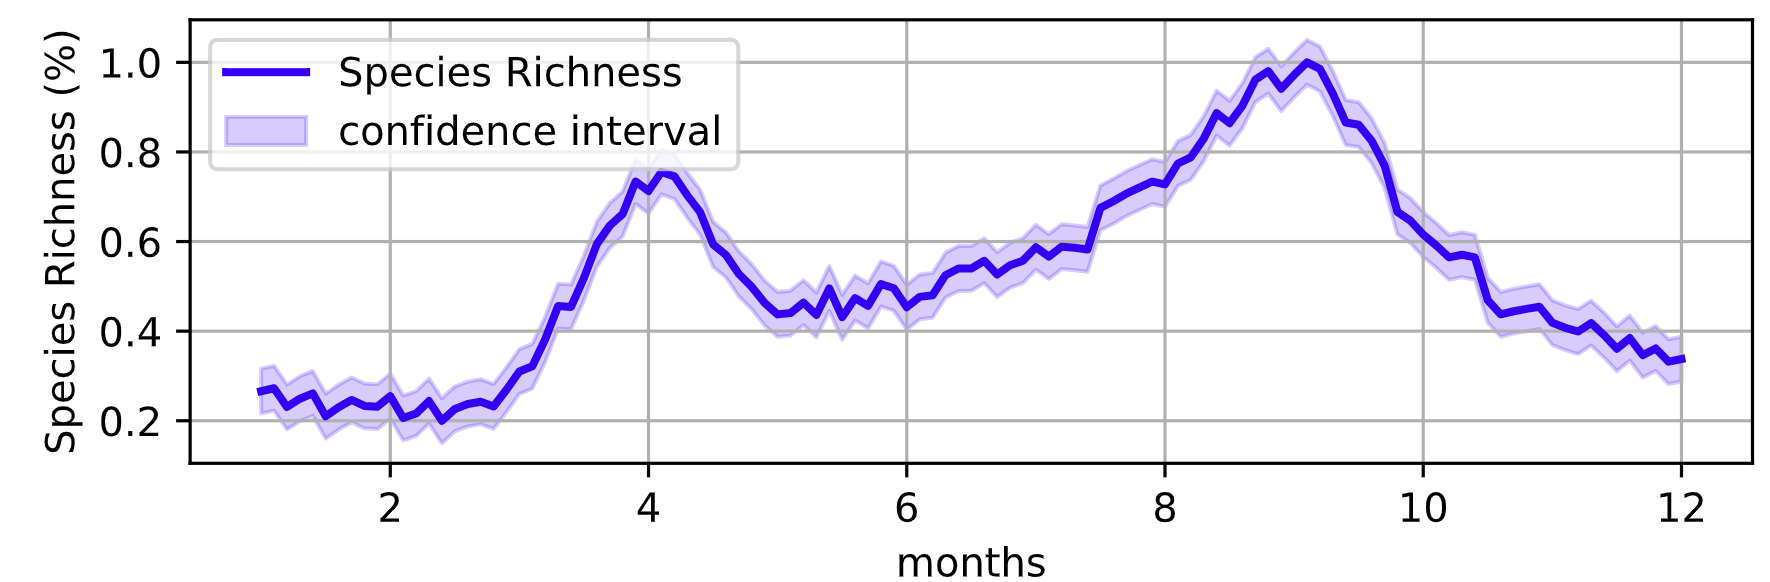
\includegraphics[width=0.7\textwidth]{./figures/basic_food_web_model_Species_Richness_Per_Year(task_1).png}
		\caption{Visualization of EEIM (in single year).}
		\label{shiboqi}
	\end{figure}
	To further calculate the biodiversity index for the region, we substitute the biomass values obtained in the previous analysis into the \textbf{Shannon Index} formula.
	\begin{equation}
		H' = - \sum_{i=1}^{S} p_i \ln(p_i)
	\end{equation}
	where $H'$ is the diversity index; $S$ is the total number of species in the ecosystem,and $p_i=\frac{Ci}{C}$ is the relative richness of species $i$.
	
	To facilitate subsequent calculations, we subjected the Shannon diversity index to standardization.
	\begin{equation}
		E = \frac{H'}{H_{\max}'} = \frac{H'}{\ln(S)}
	\end{equation}
	
	EEIM embodies significant practical meaning considering its visualization in figure \ref{shiboqi}. It can be observed that the function reaches its peaks in April and September, respectively in spring and autumn. Spring is the season to seed while autumn to harvest, both of which feature rich biodiversity. Additionally, between June and August, the crops begin to grow, nourishing numerous creatures in fields which ultimatelmately contributes to increases in species richness. When the temperature drops in January, the biodiversity reaches its bottom due to harsh living conditions. 
	
	
	\subsection{Elementary Ecology Destroyer Model, EEDM}
	\hspace{2em}In section 4.1, we propose the EEIM to model the food web under an ideal circumstance where chemical substances are excluded. In this chapter, we introduce the Elementary Ecology Destroyer Model (EEDM) to encompass humans' overuse of chemicals and corresponding negative effects on agricultural ecosystems. The final food web model which takes all the factors into consideration is made up of EEDM and EEIM.
	% 数据集构造思路
	\begin{figure}[h]
		\centering
		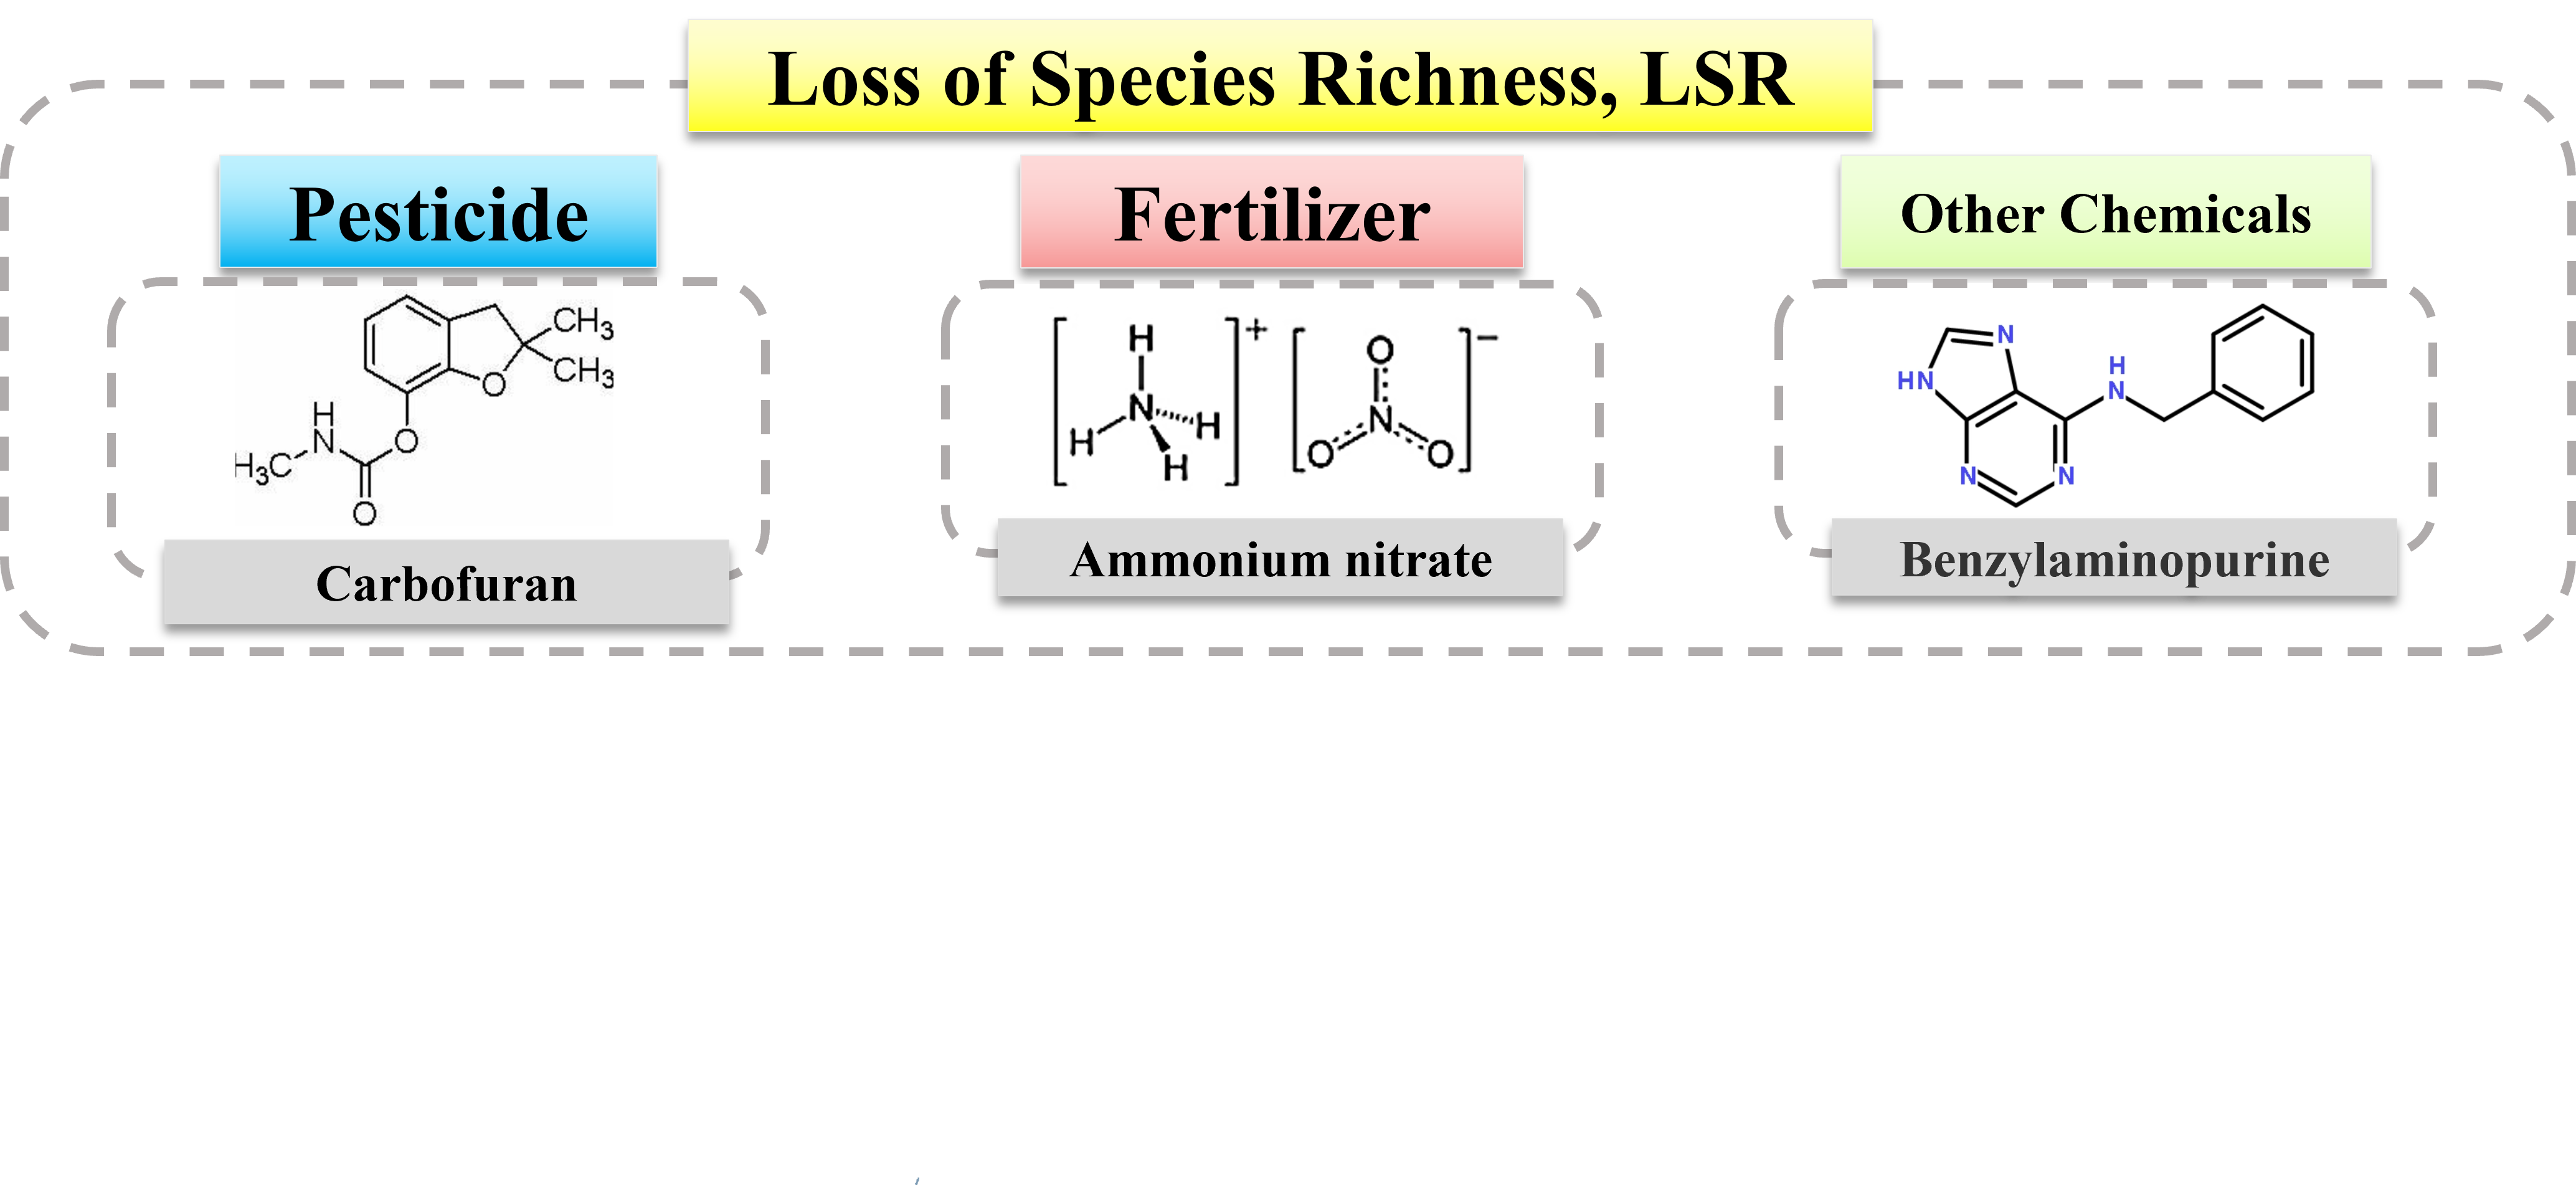
\includegraphics[width=0.8\textwidth,trim=0cm 6.2cm 0cm 0cm,clip]{./figures/dataset.png}
		\caption{Selected variables for the training dataset.}
		\label{dataset.}
	\end{figure}
	Numerous relevant researches have observed the over-complicated relationship between chemical usages and their corresponding effects. To simplify the process, we employ deep-learning methods, to be specific, the Multi-Layer-Perceptron (MLP) to better quantify the relationship between pivotal parameters and the loss of species richness. We follow a rigorous procedure to train our neural network, from dataset-preparation to robustness evaluation.
	
	
	\textbf{Dataset Preparation. }Usages of pesticides ($Pest.$), fertilizers ($Fert.$) and other chemicals ($Oths.$) are selected to be the input features, considering they are the major categories of contemporary agricultural chemicals. Loss of species richness ($LSR$) is chosen as the output label, as is illustrated in figure \ref{dataset.}. All the datas are collected from \cite{1}\cite{2}\cite{3}.
	
	% MLP的构造思路
	\begin{figure}[h]
		\centering
		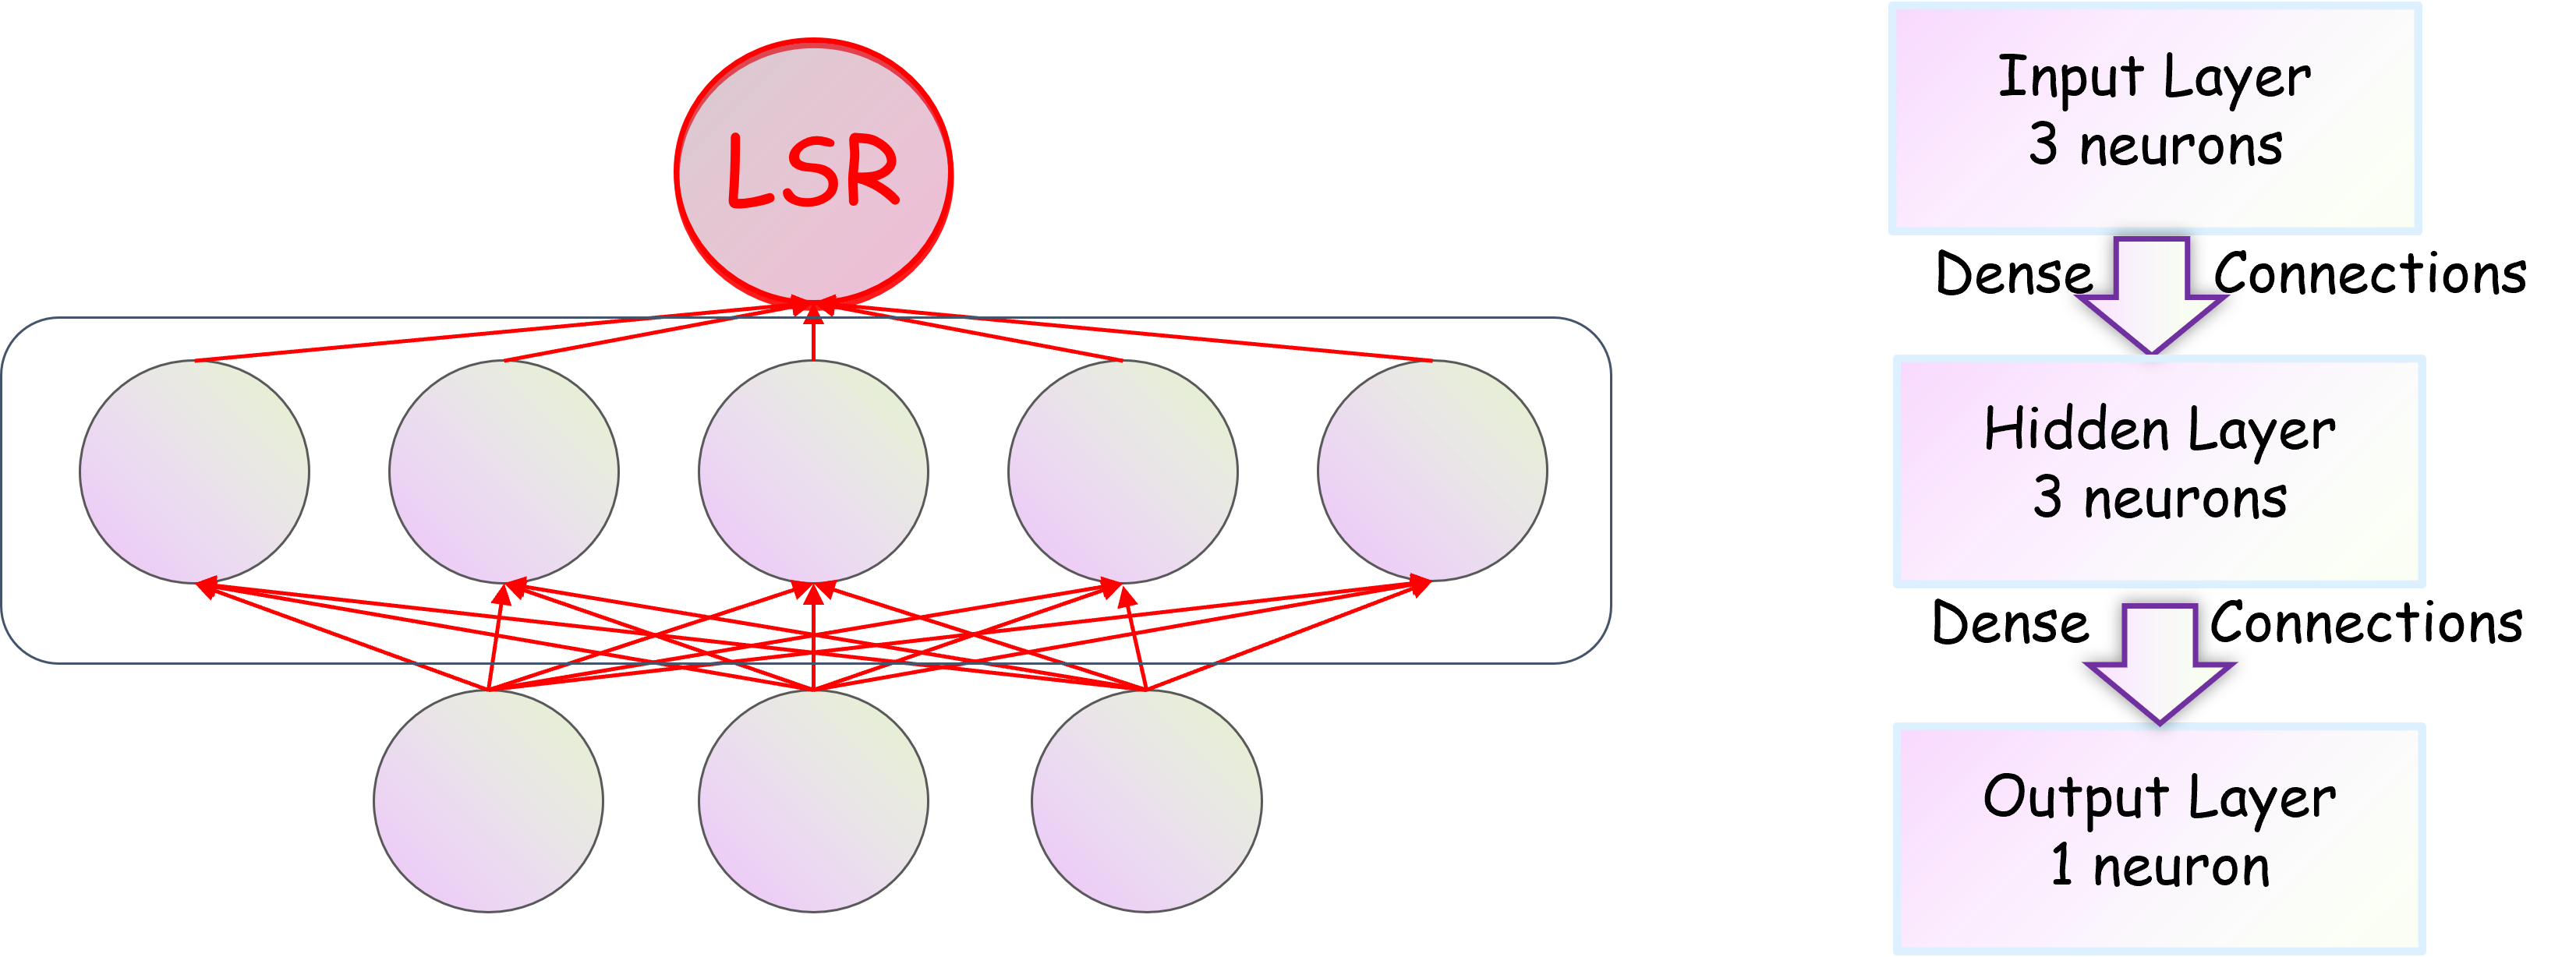
\includegraphics[width=0.6\textwidth]{./figures/MLP.png}
		\caption{Backbone MLP structure of the EEDM.}
		\label{MLP}
	\end{figure}
	
	\textbf{Experimental Configuration. }We applied one RTX 4060 GPU as hardware platform and the PyTorch Deep-Learning Framework. Mean Squared Loss (MSE) and Small Gradient Descents (SGD) are chosen respectively as loss function and optimization algorithm, as is shown in equation \ref{optimization}. Hyper-parameters are configured as: $batch\_size=16,\ epochs=125,\ learning\_rate=0.001$. Additionally, regularization techniques are employed to mitigate over-fitting: $dropout\_ratio=0.2$. Finally, we designed a 3-3-1 neuron distribution for MLP (figure \ref{MLP}), which could be expressed as equation \ref{fp}, where $\textbf{W}_1\in\mathbb{R}^{3\times3},\textbf{W}_2\in\mathbb{R}^{1\times3},\textbf{b}_1\in\mathbb{R}^{3\times1},\textbf{b}_2\in\mathbb{R}^{1\times1},\sigma(\cdot)\in\mathbb{R}^{3\times3}$
	
	% 损失函数和优化算法
	\begin{equation}
		L(\textbf{w},b)=\frac{1}{n}\sum_{i=1}^{\mathbb{B}}\frac{1}{2}(\textbf{w}^T\textbf{x}^{(i)}+b-y^{(i)})^2,\hspace{0.3em}(\textbf{w},b)\leftarrow(\textbf{w},b)-\frac{\eta}{|\mathcal{B}|}\sum_{i\in\mathcal{B}}\partial_{(\textbf{w},b)}l^{(i)}(\textbf{w},b).
		\label{optimization}
	\end{equation}
	
	% MLP基本原理
	\begin{equation}
		\begin{cases}
			\textbf{O} = \sigma(\textbf{W}_1\cdot\textbf{X}+\textbf{b}) \\
			LSR = \textbf{W}_2\cdot\textbf{O} + \textbf{b}
		\end{cases},\hspace{0.2em}\text{where}\hspace{0.2em}\sigma(\cdot)=\mathrm{ReLU(\cdot)}
		\label{fp}
	\end{equation}
	
	We further processed equation \ref{fp} to transform it linearly, which goes as:
	\begin{equation}
		LSR = \textbf{W}_{total}\cdot\textbf{X}+b_{total},\hspace{0.2em}\text{where}\hspace{0.2em}\begin{cases}
			\textbf{W}_{total} = \textbf{W}_2\cdot\sigma(x_i)\cdot\textbf{W}_1 \\
			\textbf{b}_{total} = \textbf{W}_2\cdot\sigma(x_i)\cdot\textbf{b}_1 + \textbf{b}_2
		\end{cases}
	\end{equation}
	
	Through training (figure \ref{t}) we acquire the primitive form of EEDM:
	\begin{align}
		& \begin{cases}
			\textbf{W}_{total} = \begin{pmatrix}
				-0.263 \\ 0.273 \\ -0.288
			\end{pmatrix}^{\top}\cdot\begin{pmatrix}
				1 & 0 & 0 \\
				0 & 1 & 0 \\
				0 & 0 & 1
			\end{pmatrix}\cdot\begin{pmatrix}
				-0.295 & -0.281 & -0.322 \\
				0.307 & 0.263 & 0.323 \\
				-0.282 & -0.258 & -0.310
			\end{pmatrix}=\begin{pmatrix}
				0.243 \\ 0.220 \\ 0.262
			\end{pmatrix}^{\top} \\
			\textbf{b}_{total} = \begin{pmatrix}
				-0.263 \\ 0.273 \\ -0.288
			\end{pmatrix}^{\top}\cdot\begin{pmatrix}
				1 & 0 & 0 \\
				0 & 1 & 0 \\
				0 & 0 & 1
			\end{pmatrix}\cdot\begin{pmatrix}
				-0.174 \\ 0.179 \\ -0.167
			\end{pmatrix}+(0.103) = 0.246
		\end{cases} \\
		& \xrightarrow{}LSR(\%) = 0.243\times Pest.(kg/ha) + 0.220\times Fert.(kg/ha) + 0.262\times Oths.(kg/ha) + 0.246
		\label{primitive}
	\end{align}
	where $LSR$ if the loss of species richness, $Pest.$, $Fert.$, $Oths.$ respectively stands for the quantity of used pesticides, fertilizers and other chemicals.
	% 训练图
	\begin{figure}[htbp]
		\centering
		\begin{subfigure}{0.35\textwidth}
			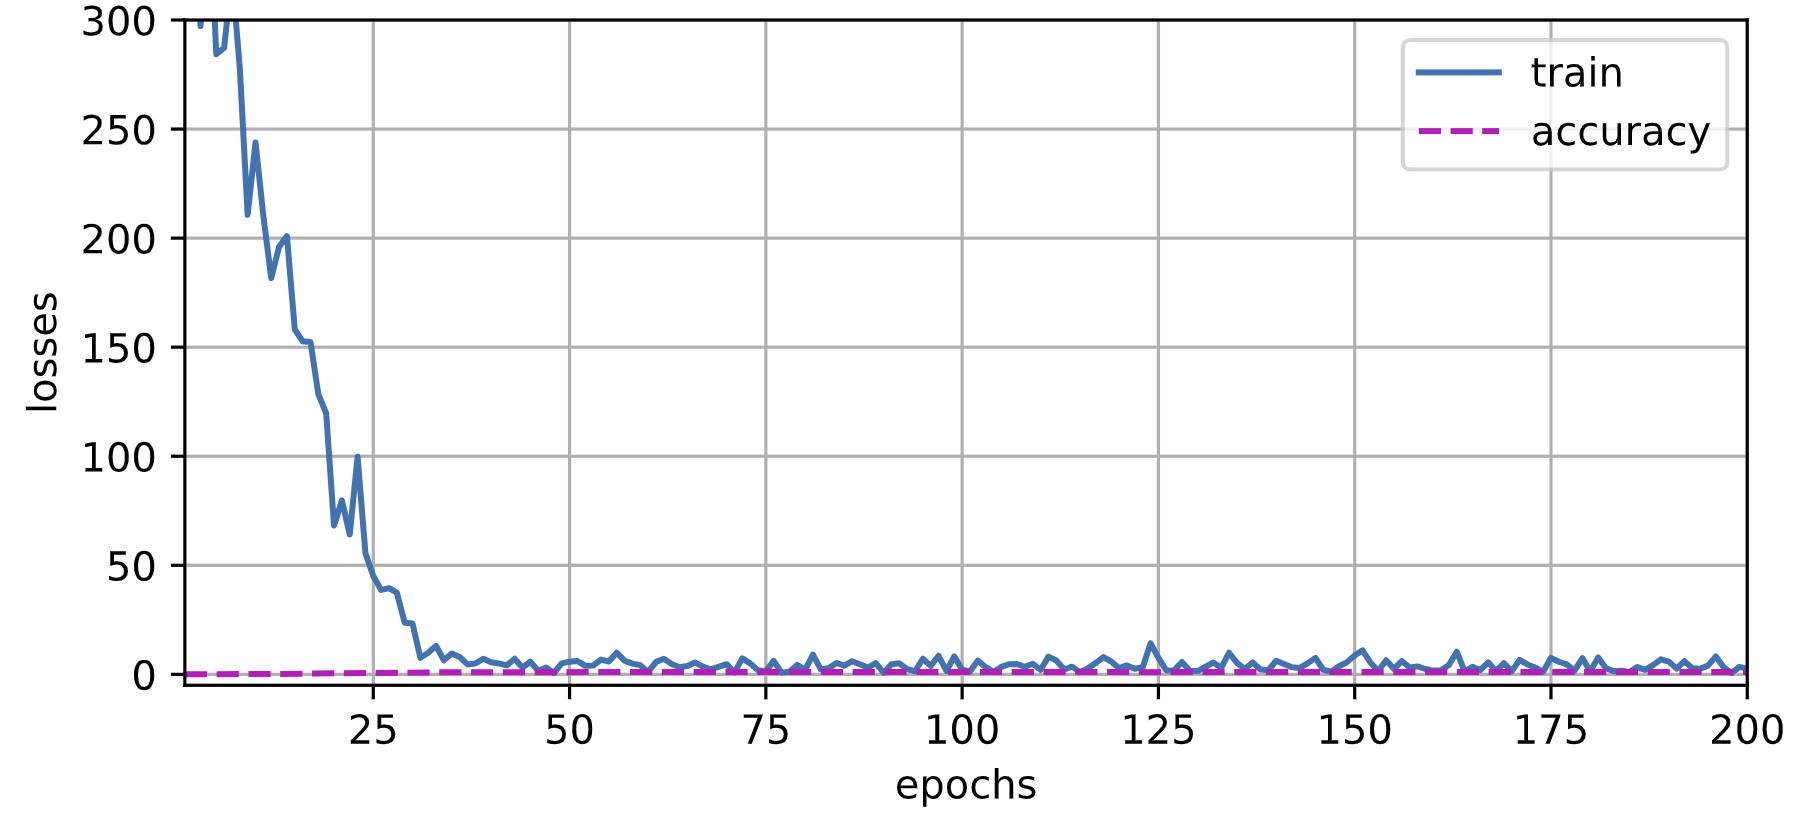
\includegraphics[width=\textwidth,trim=0cm 1.5cm 0cm 0cm,clip]{./figures/train.png}
			\label{train}
		\end{subfigure}
		\begin{subfigure}{0.35\textwidth}
			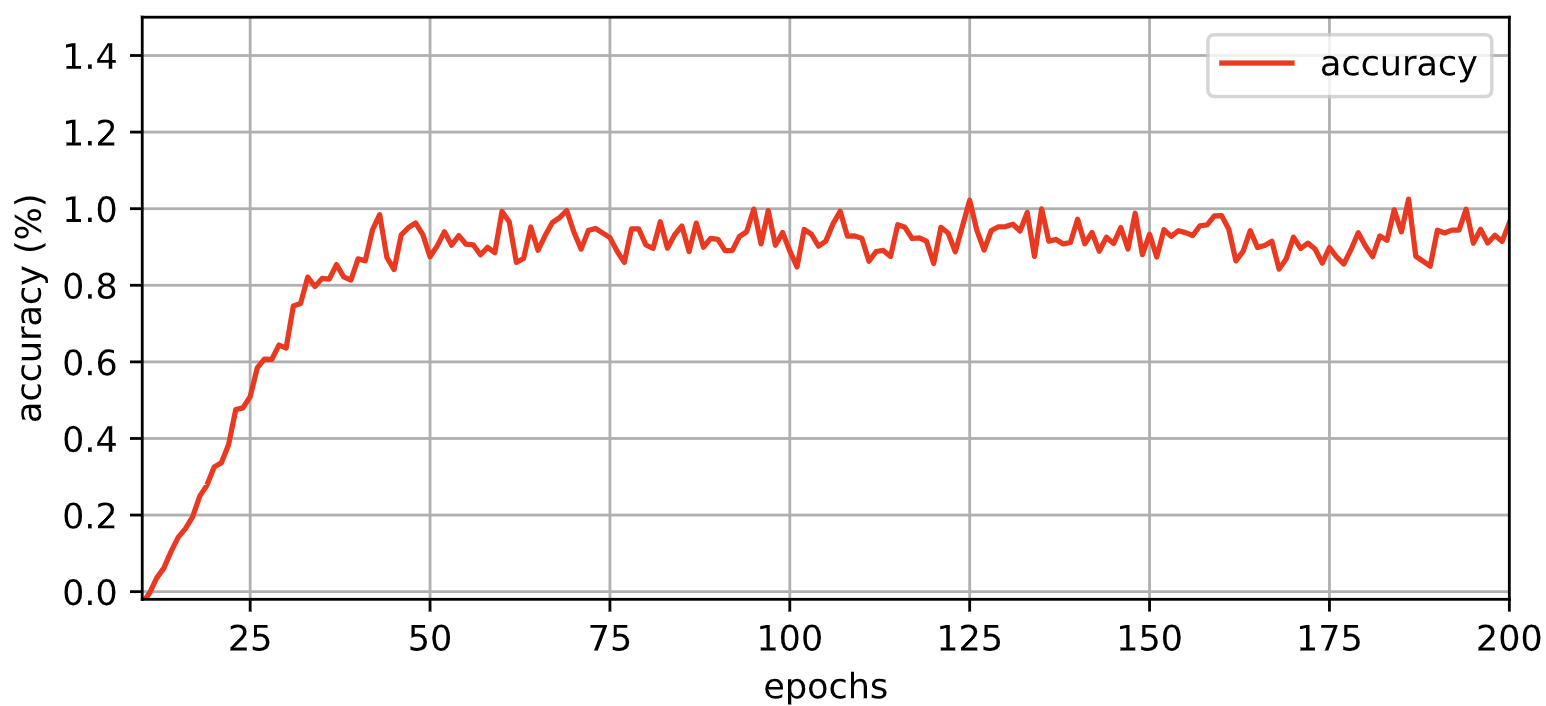
\includegraphics[width=\textwidth,trim=0cm 1.5cm 0cm 0cm,clip]{./figures/accuracy.png}
			\label{test}
		\end{subfigure}
		\caption{Our model-training process.}
		\label{t}
	\end{figure}
	
	A deeper optimization is conducted by mapping EEDM (equation \ref{primitive}) to time-dimension. Considering each of its sub-variables as functions correlated to time, we use \textbf{MATLAB} to fit each equation, culminating in a time-based EEDM (equation \ref{time}, figure \ref{ti}):
	\begin{align}
		&LSR = \begin{pmatrix}
			\alpha(t) \\ \beta(t) \\ \theta(t)
		\end{pmatrix}=
		\begin{pmatrix}
			-0.0012619\times t^2+5.1116424\times t-5176.717 \\
			-0.06358907\times t^2+257.34633611\times t-260251.460 \\
			-0.001238\times t^2+5.02035714\times t-5087.3170
		\end{pmatrix} \\
		& \xrightarrow{ }LSR = -0.01462044487\times t^2+59.17365663\times t-59845.89449
		\label{time}
	\end{align}
	
	\begin{figure}[h]
		\centering
		\begin{subfigure}{0.3\textwidth}
			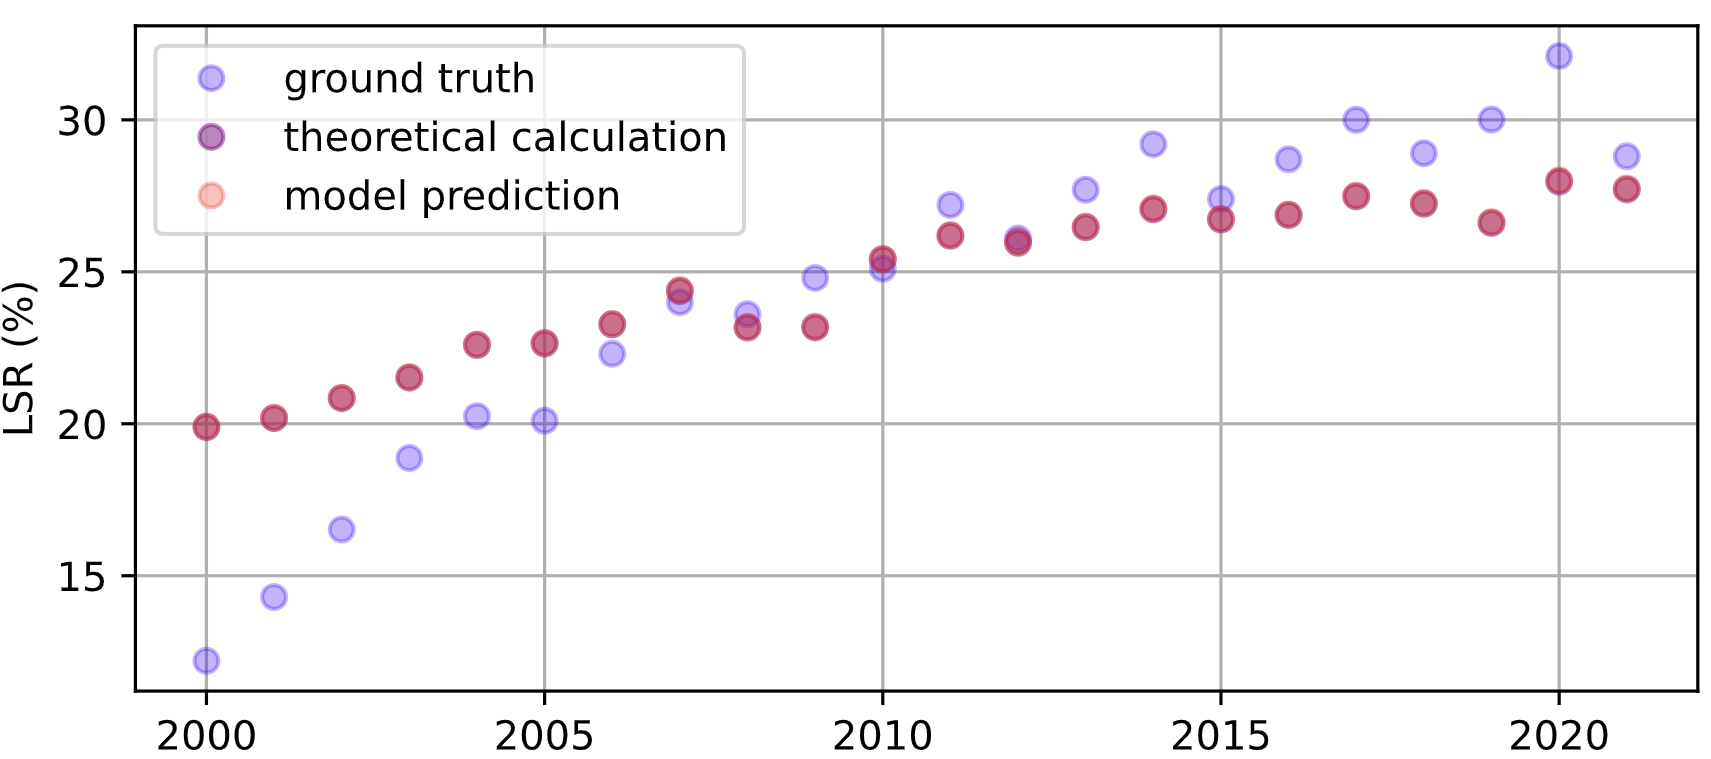
\includegraphics[width=\textwidth]{./figures/LSR_primitive_dimension.png}
			\caption{Primitive Form.}
		\end{subfigure}
		\begin{subfigure}{0.3\textwidth}
			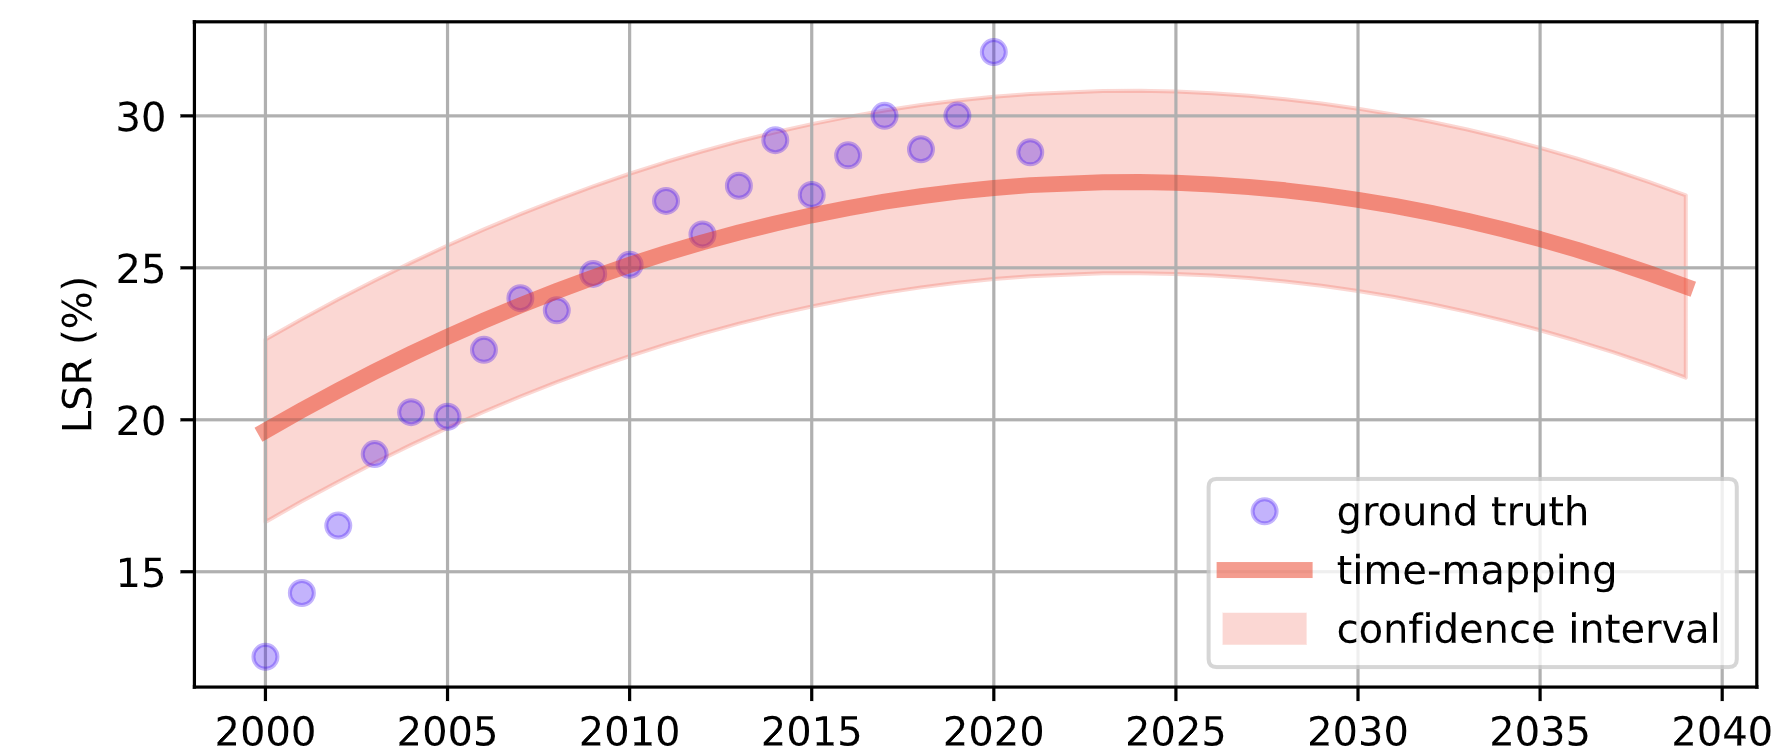
\includegraphics[width=\textwidth]{./figures/LSR_time_dimension.png}
			\caption{Time-dimension Form}
		\end{subfigure}
		\caption{Two forms of the EEDM: primitive and time-based respectively.}
		\label{ti}
	\end{figure}
	
	From figure \ref{t} it can be observed that our model reaches an accuracy of 90.3\%. We further validated our model by measuring the specific effects of chemical usages on birds population and the insects counterparts, as is illustrated in figure \ref{chemics}. It can be seen that overuse of chemicals contributes the greatest losses in plants richness, followed by insects. Such prediction aligns with reality since plants are the dominant creatures in agricultural ecosystems and insects are essential pollinators for crops.
	
	\begin{figure}[h]
		\centering
		\begin{subfigure}[b]{0.43\textwidth}
			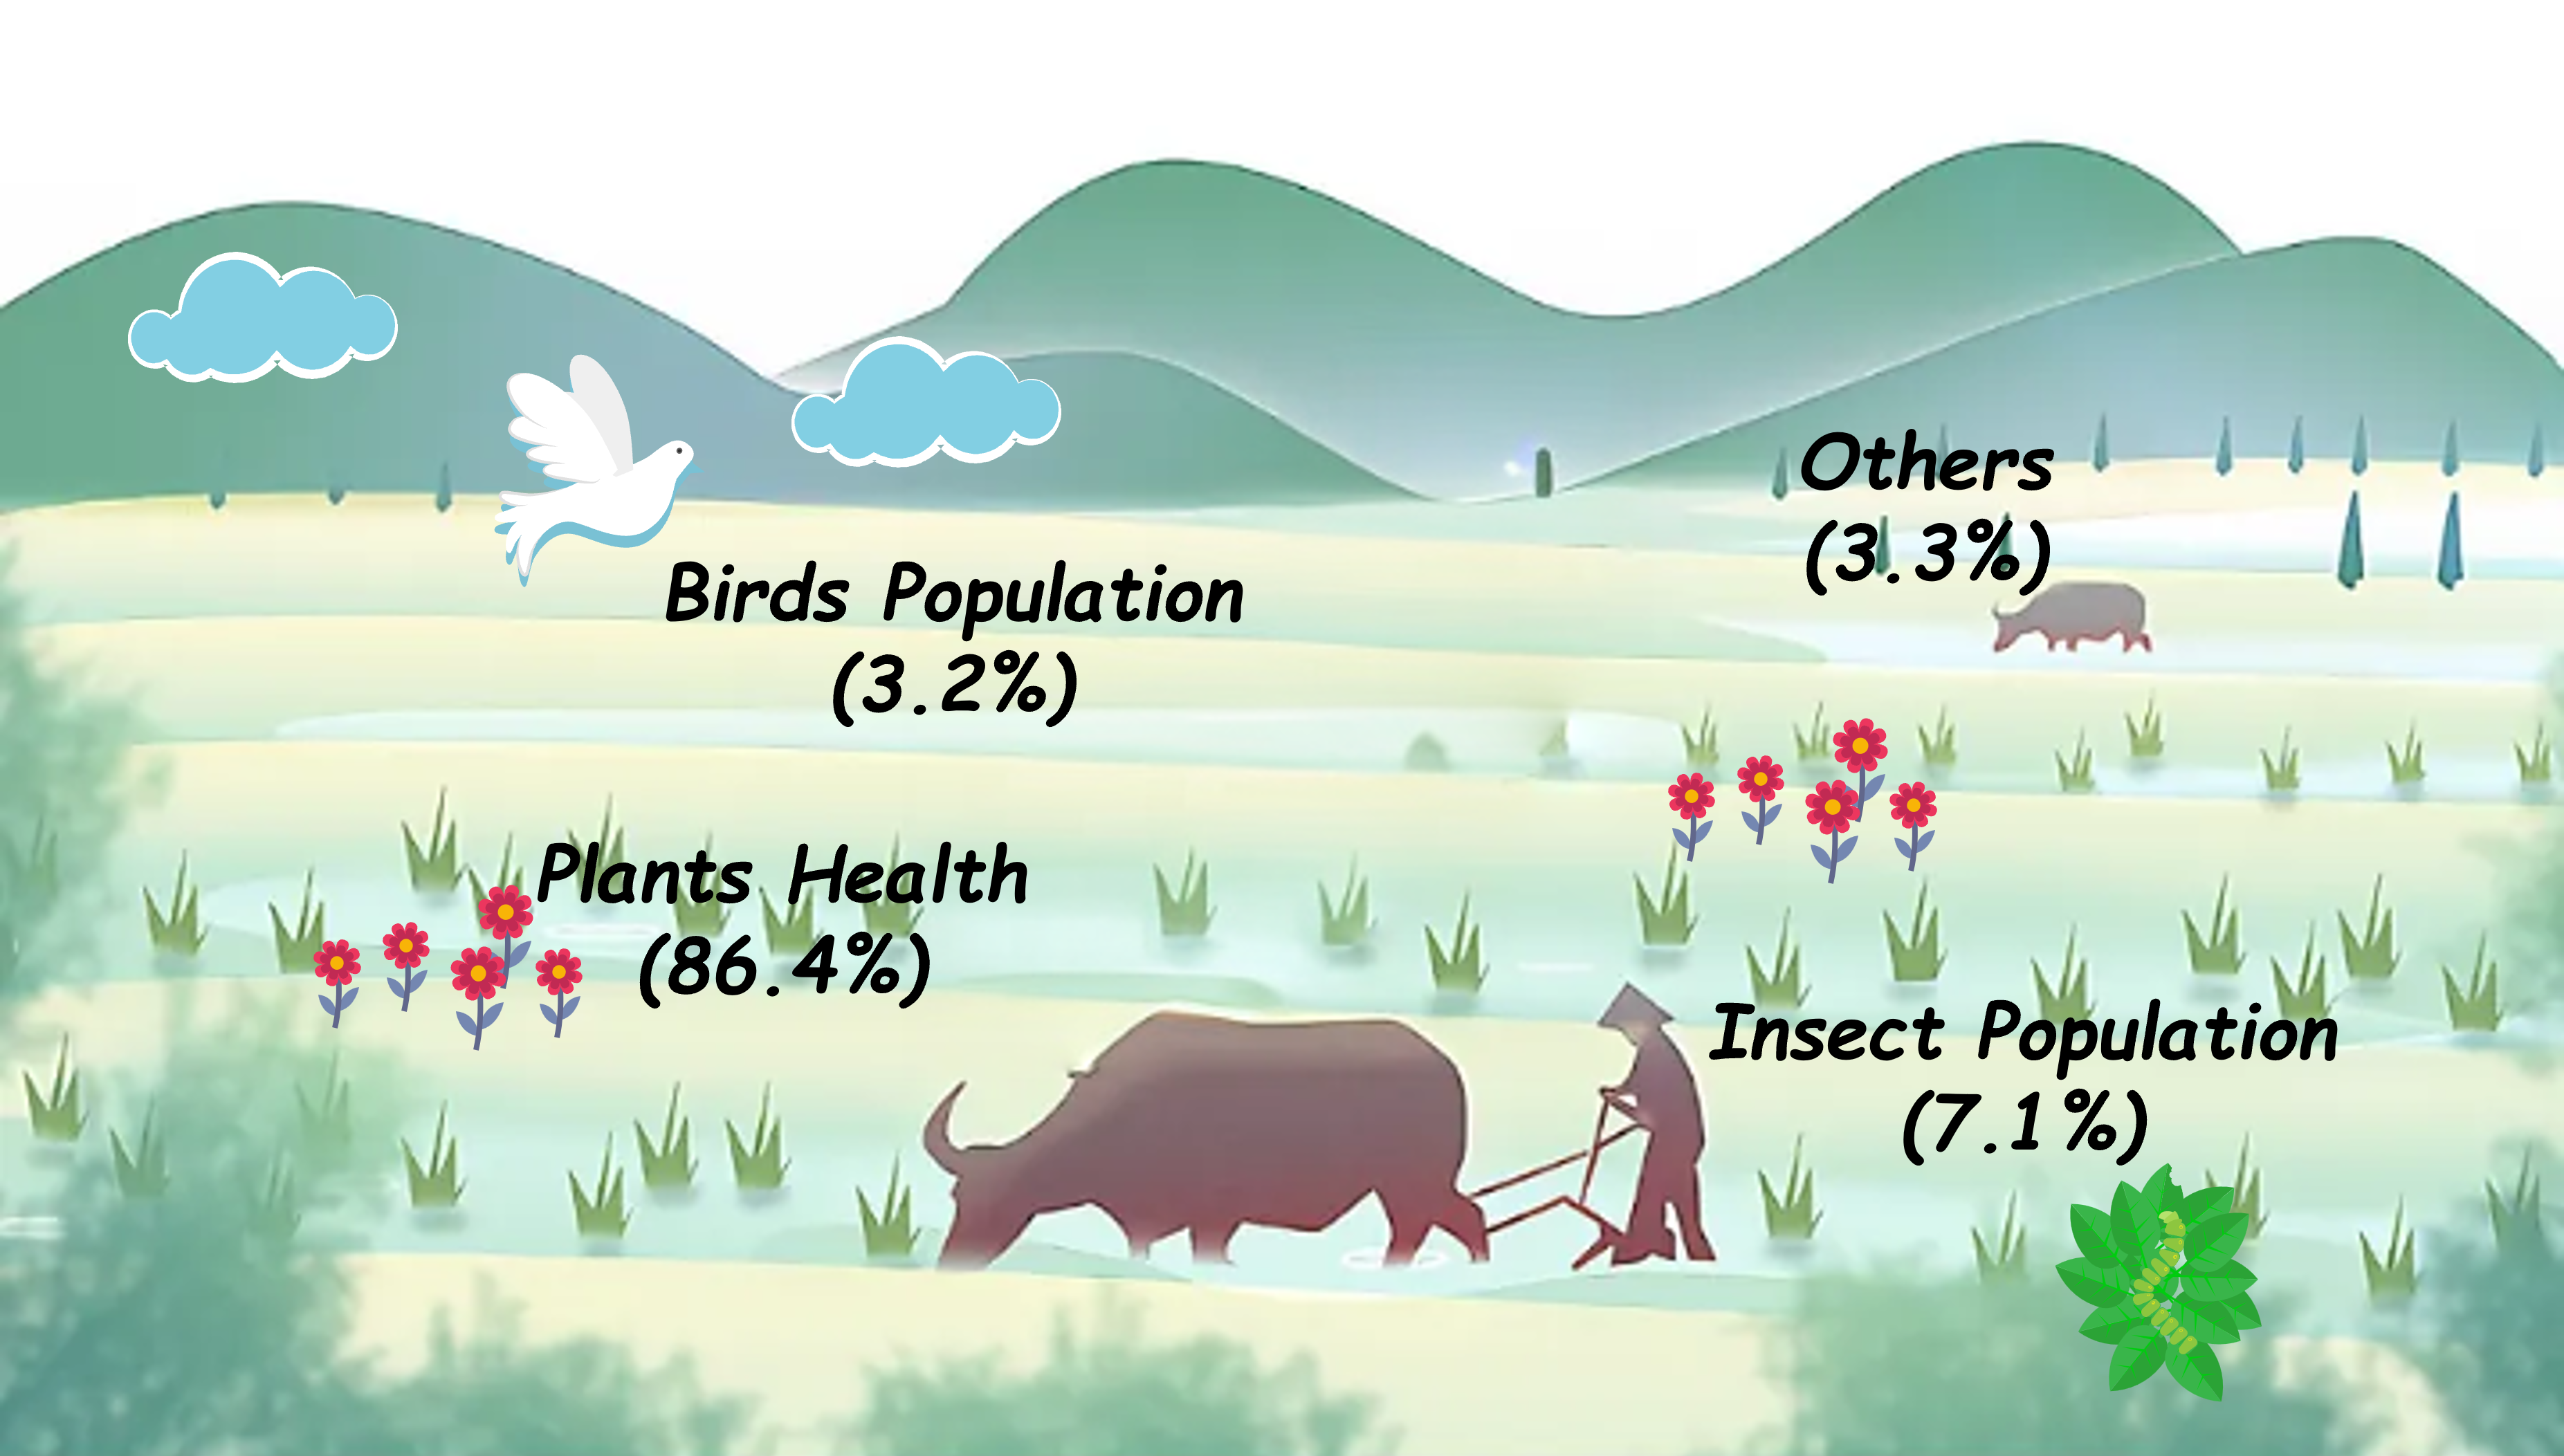
\includegraphics[width=\textwidth]{./figures/chemics on eco(task 1).png}
			\caption{Agricultural ecosystem.}
		\end{subfigure}
		\begin{subfigure}[b]{0.36\textwidth}
			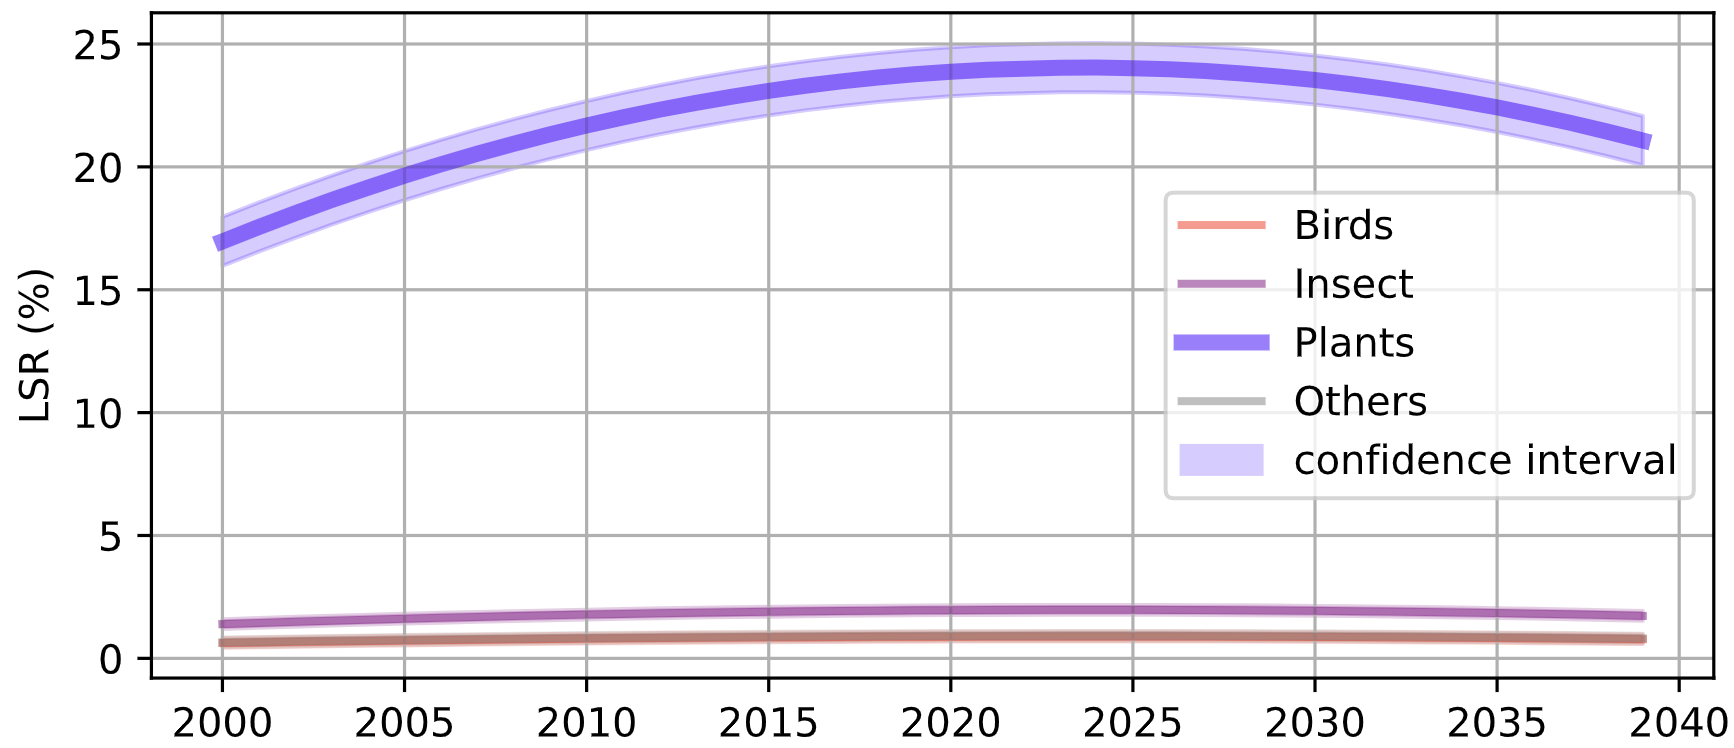
\includegraphics[width=\textwidth]{./figures/impacts_on_birds_etc(task 1)}
			\caption{Loss of species richness.}
		\end{subfigure}
		\caption{Effects of chemical usages on agricultural ecosystems.}
		\label{chemics}
	\end{figure}
	\subsection{Food Web Model}
	
	
	%%%%%%%%%%%%%%%%%%%%%%%%第二题
	\section{Reemergence of native species---\textit{``They Are Home''}}
	\hspace{2em}Edge habitats sit in the buffer zone between agricultural fields and surrounding ecosystems. Considering that our research focus is forest-to-farm situations, we assume the surrounding ecosystems are natural forests. In this section, we applied the broadened version of Pascal's Triangle and Ecosystem Stability Model to evaluate impacts of native species' reemergence, which offer a dynamic view on the complete process of ecosystem evolution.
	\subsection{Pascal's Triangle is all you need}
	\hspace{2em}Native species are considered to have migrated into edge habits due to human exploits on the primary evolution stage of agricultural ecosystems. Therefore, they feature strong seasonal dynamics and geographical movements.
	
	Pascal's Triangle is a triangular array of number which is widely used in algebra. Notice that the shape follows an increasing trend from inside out, we utilize this characteristic to demonstrate the geographical distributions of native species in terms of diverse evolution stages. By concatenating two triangles together into a square, we have the broadened Pascal's Triangle, which goes as:
	\begin{equation}
		\begin{matrix}
			& & & &1 & & & & \\
			& & &1&  &1& & & \\
			& &1& &2 & &1 & & \\
			&1& &3&  &3&  &1 & \\ 
			&1& &3&  &3&  &1 & \\ 
			& &1& &2 & &1 & & \\
			& & &1&  &1& & & \\
			& & & &1 & & & & \\
		\end{matrix}\hspace{0.2em} \iff\hspace{0.3em}C(n,k)_x=C(n,k)_y=\frac{n!}{k!(n-k)!}\iff\begin{pmatrix}
			C_x \\C_y
		\end{pmatrix}
	\end{equation}
	
	Similarly, by taking reciprocal on each value, we acquire another version of Pascal's Triangle which could be applied to explain the intermediate evolution periods when the majority of native species distribute in edge habitats: $\begin{pmatrix}
		\frac{1}{C_x} & \frac{1}{C_y}
	\end{pmatrix}$. Visualization of both Pascal's Triangle is illustrated in figure \ref{tr}.
	% 这是杨辉的两种形式
	\begin{figure}[h]
		\centering
		\begin{subfigure}{0.25\textwidth}
			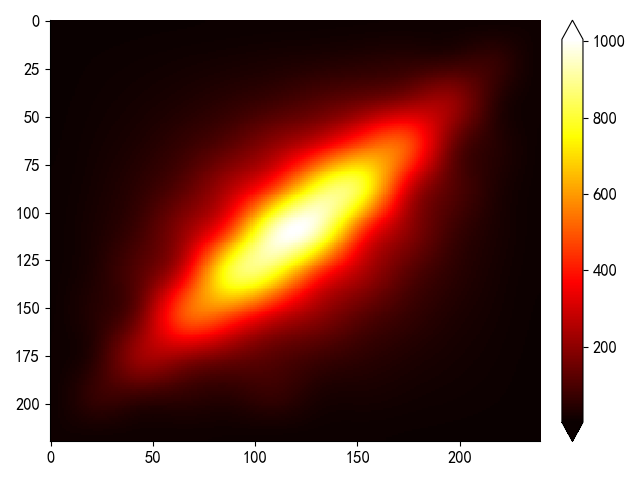
\includegraphics[width=\textwidth]{./figures/primitive triangle(task2).png}
			\caption{Primitive form.}
			\label{p}
		\end{subfigure}
		\begin{subfigure}{0.25\textwidth}
			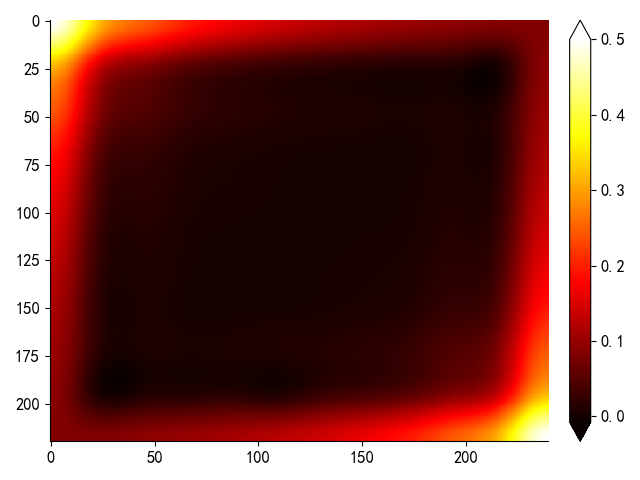
\includegraphics[width=\textwidth]{./figures/primitive reprocical triangle(task2)}
			\caption{Reciprocal form.}
			\label{wobuxaingxiele}
		\end{subfigure}
		\caption{Broadened Pascal's Triangle, where a brighter color indicates a larger species richness.}
		\label{tr}
	\end{figure}
	
	What differs \ref{p} and \ref{wobuxaingxiele} is their application scenarios. Figure \ref{p} describes the elementary stage of agricultural ecosystem evolution where the majority of native species distribute in central regions featuring sufficient living resources; Figure \ref{wobuxaingxiele} demonstrates the middle periods of evolution where the human exploits get involved and are transforming it into an agricultural ecosystem. Native species are accordingly compelled to migrate into edge habitats. 
	\subsection{Impacts of reemergence of native species}
	\hspace{2em}The migration process is firstly simulated using our Broadened Pascal's Triangle. It's worth noting that, instead of choosing two specific species, we select symbolic creatures of two categories, namely $A$ and $B$, to generalize our model. Species $A$ is a native insect featuring dense population (such as \textit{Apis Mellifera}) while $B$ is a local animal with long lifespan but relatively low population (such as \textit{Cervus Elaphus}). 
	
	As is illustrated in figure \ref{mig}, the triple periods of ecosystem evolution are demonstrated, including stage 1 (Natural Forest Area), stage 2 (Converted Agricultural System) and stage 3 (Mature Ecosystem). In stage 1, $A$ and $B$ settle in central regions; In stage 2, they migrated into edge habitats temporarily to escape human interference,; In stage 3, due to a flourished and mature agricultural system, both species reemerged and relocated, sharing the living resources with human beings.
	\begin{figure}[h]
		\centering
		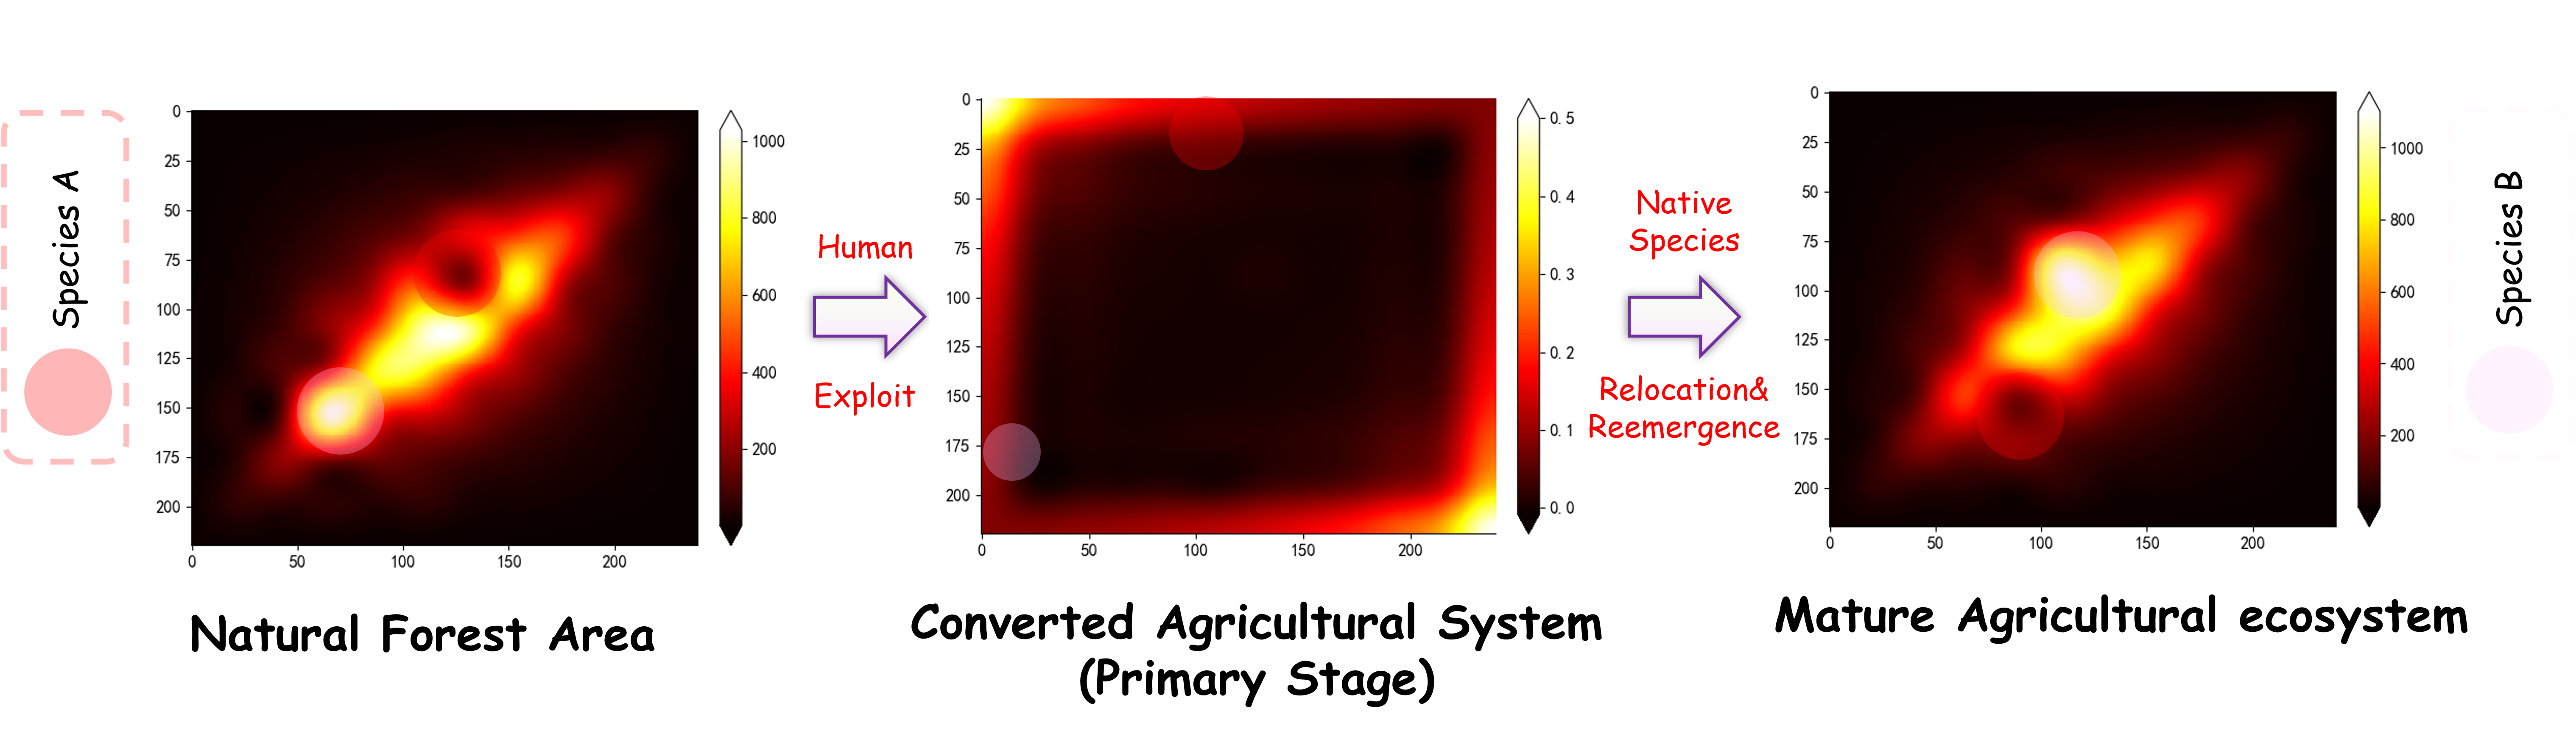
\includegraphics[width=\textwidth]{./figures/reemergence(task 2).png}
		\caption{Three stages in ecosystem evolution and native species' reemergence.}
		\label{mig}
	\end{figure}
	
	While the Broadened Pascal's Triangle describes the dynamic reemergence of native species, the Ecosystem Stability Model (ESM) reveals the exact influence of species' reemergence on overall ecosystem stability. 
	
	ESM is composed of Resilience Stability ($RLS$) and Resistant Stability ($RTS$), both of which are correlated with species richness or diversity. Therefore, the reemergence of  $A$ and $B$ directly positively impacts the ecosystem by contributing to $RLS$ and $RTS$.
	
	\begin{figure}[h]
		\centering
		\begin{subfigure}[b]{0.46\textwidth}
			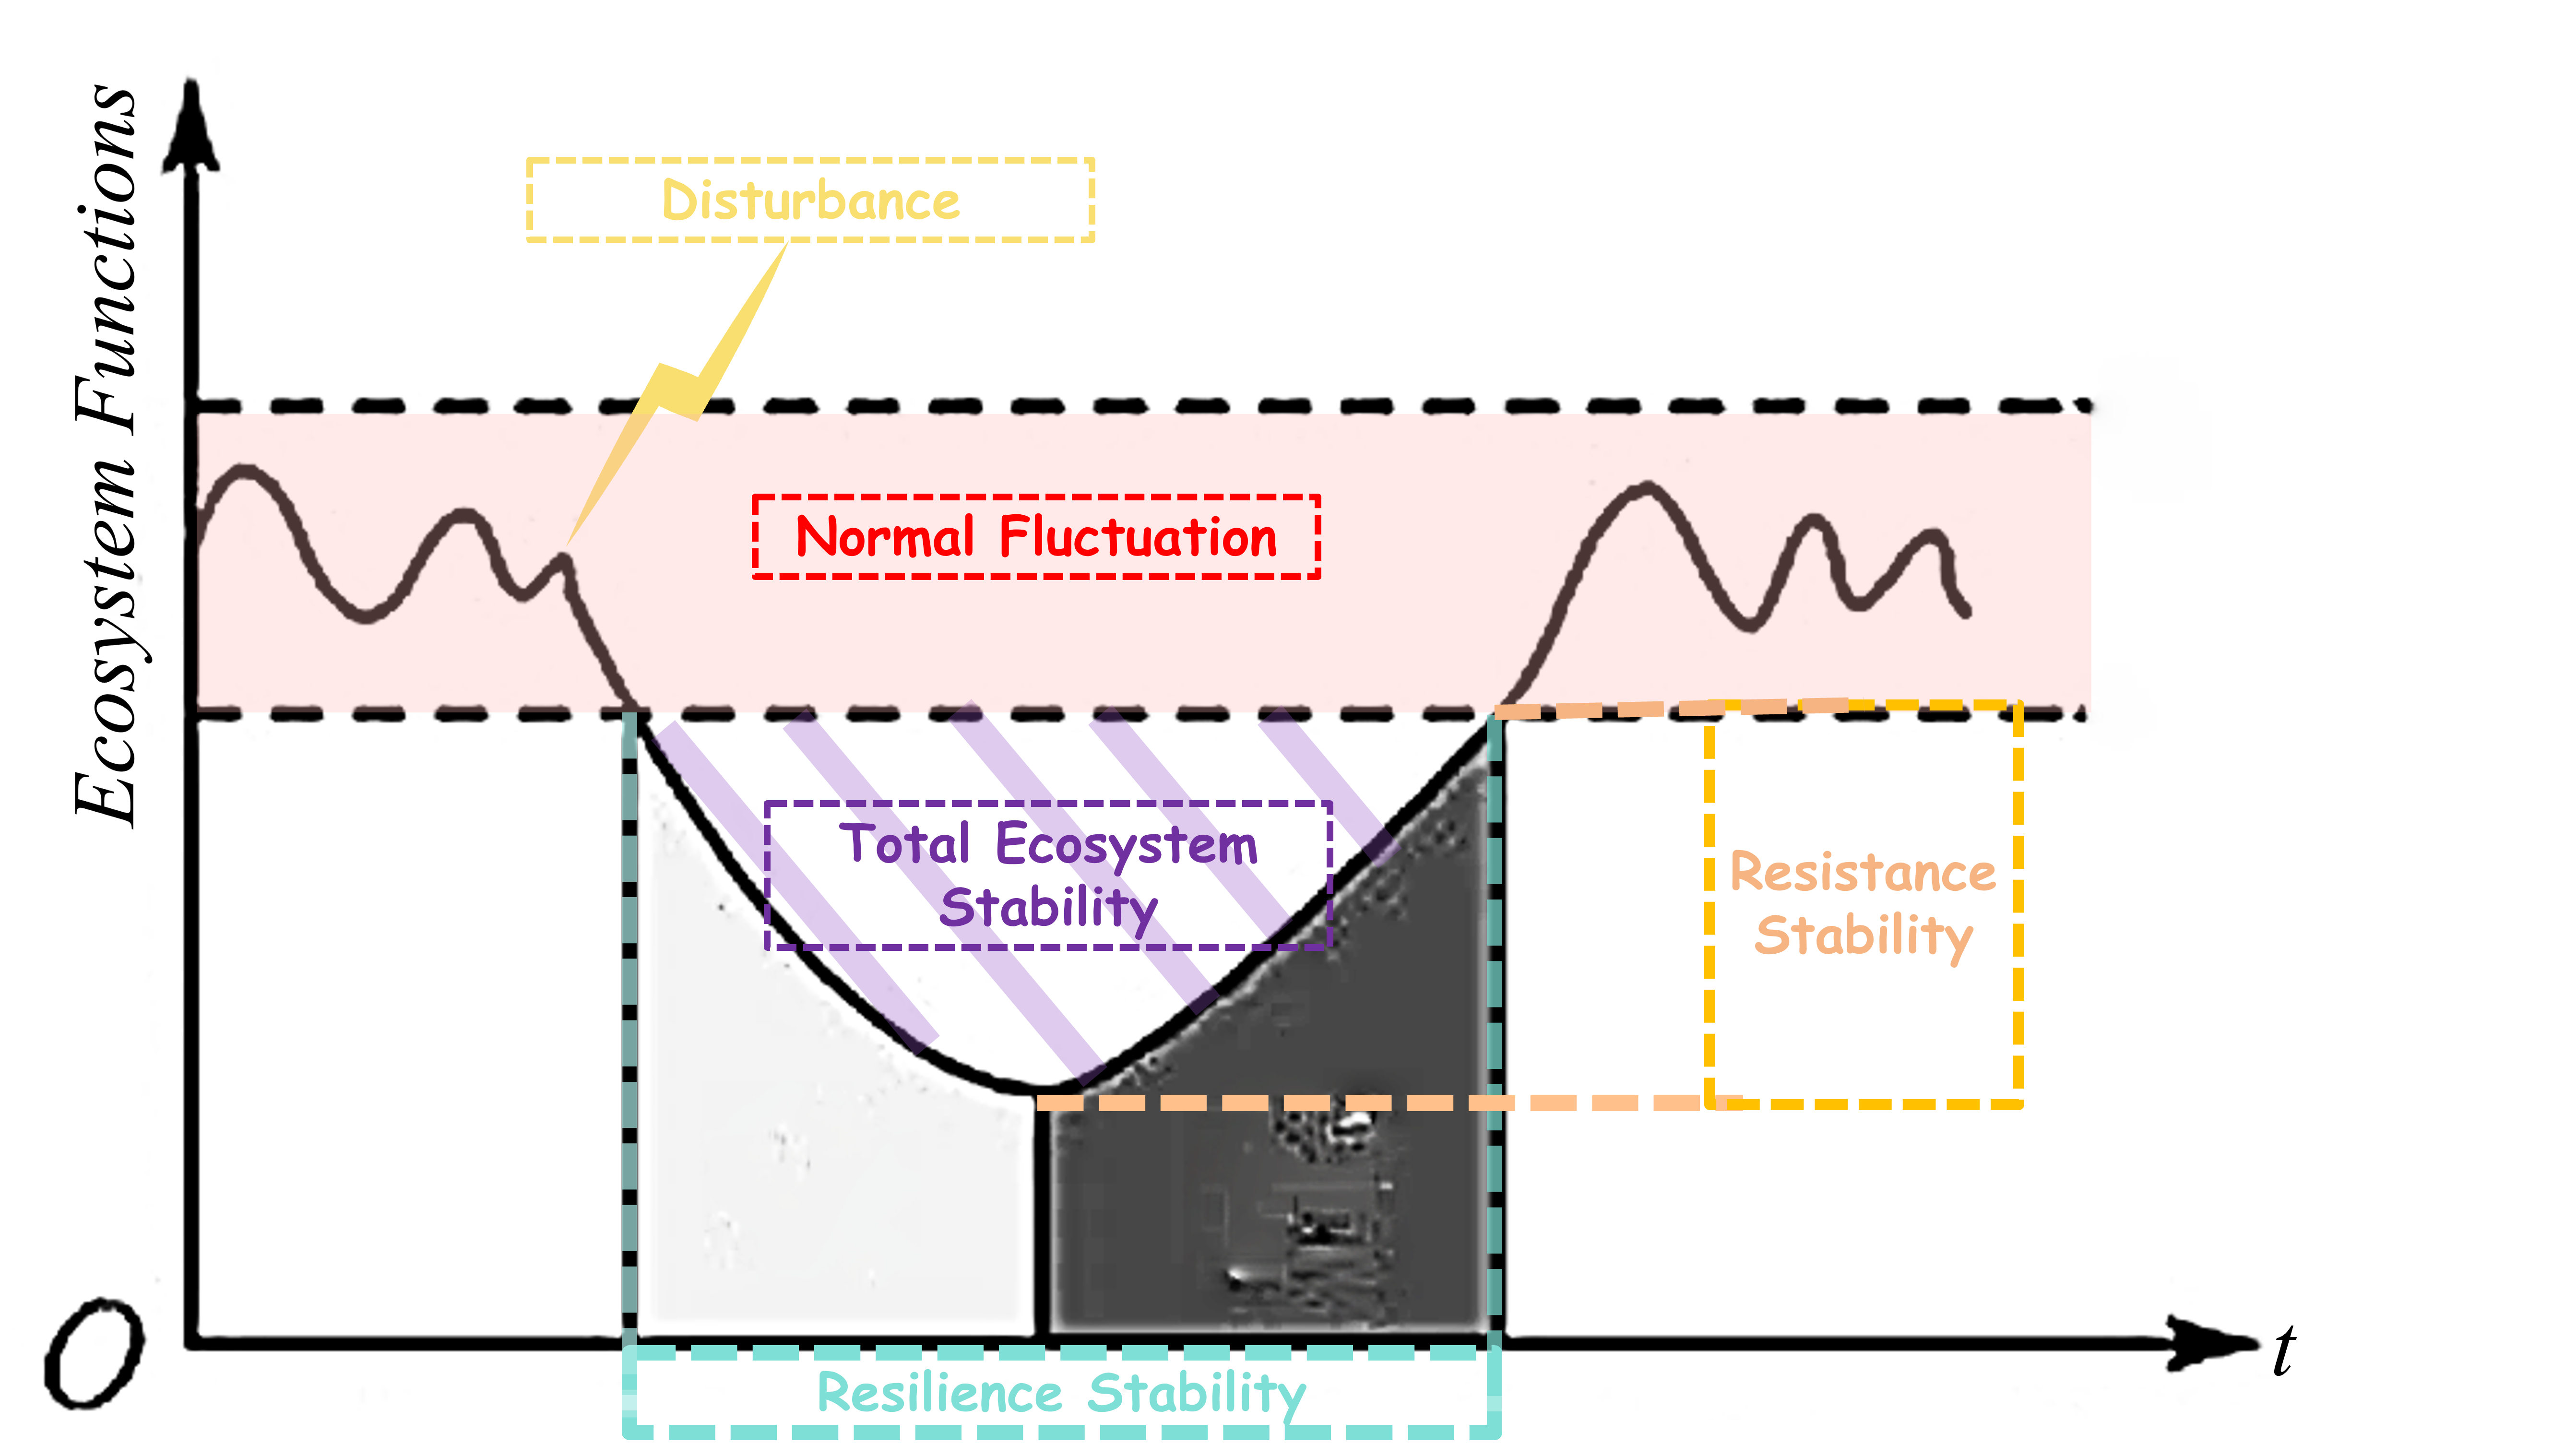
\includegraphics[width=\textwidth]{./figures/stability(task2).png}
			\caption{Ecosystem Stability Model.}
			\label{hhh}
		\end{subfigure}
		\begin{subfigure}[b]{0.44\textwidth}
			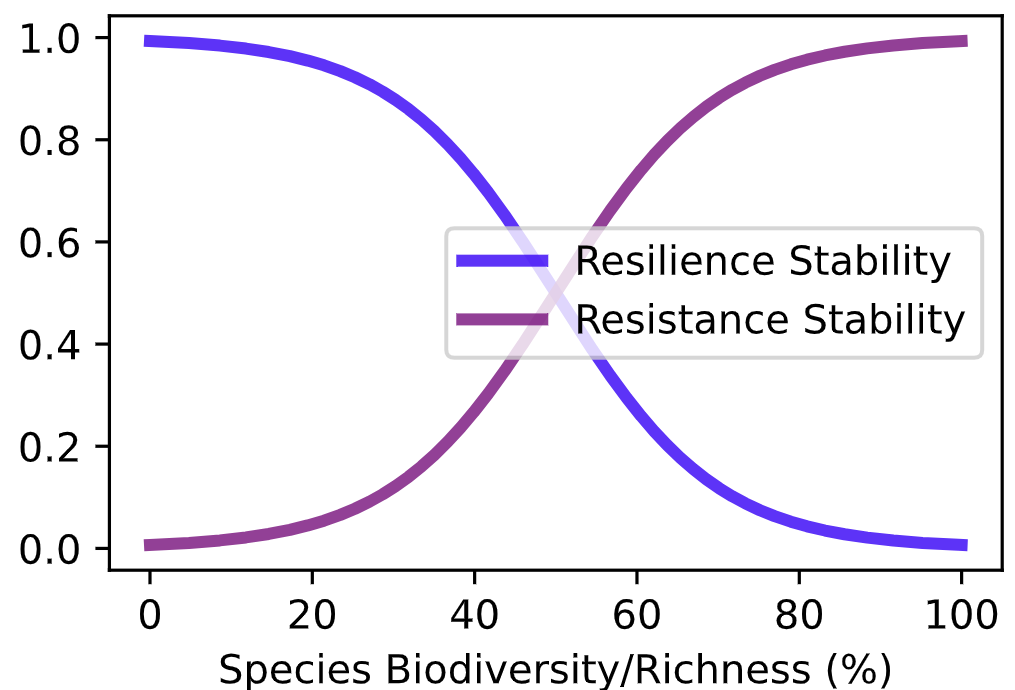
\includegraphics[width=\textwidth]{./figures/RSES(task 2).png}
		\end{subfigure}
		\caption{Illustrations of the ESM Model.}
	\end{figure} 
	
	Let a sudden disturbance occur in ecosystem (given in figure \ref{hhh}). Define $Thresh_{min}$ as the minimum threshold of functional fluctuation in a stable ecosystem, while $F$ as ecosystems' function, $t_0$ and $t_1$ respectively the first, second time when $Thresh_{min}=F$. Therefore we have:
	\begin{equation}
		\begin{cases}
			TES = \int_{t_0}^{t_1}(Thresh_{min}-F) \\
			RTS = Thresh_{min} - \min{F} \\
			RLS = t_1 - t_0
		\end{cases},\text{and}\begin{cases}
			Stability \propto \frac{1}{TES} \\
			RTS \propto Richness \\
			RLS \propto \frac{1}{Richness}
		\end{cases}
	\end{equation}
	
	A more detailed analysis is conducted. Assign $Richness_{before}$ to represent the species richness before the reemergence of $A$ and $B$, while $Richness_{after}$ the opposite. Obviously we have: $Richness_{after}>Richness_{before}$, considering $Thresh_{min}$ as a constant, we have:
	\begin{align*}
		& \begin{cases}
			RTS_{after}>RTS_{before} \\
			RLS_{after}<RLS_{before} \\
		\end{cases} \xrightarrow{ }\begin{cases}
			F_{after}>F_{before} \\
			(t_1-t_0)_{after}<(t_1-t_0)_{before}
		\end{cases}\xrightarrow{ }TES_{after}<TES_{before} \\
		&\xrightarrow{ } Stability_{after}>Stablity_{before}
	\end{align*}
	
	Therefore, we reach to the conclusion that reemergence of species $A$ and $B$ improved the overall stability of mature agricultural ecosystem. Additionally, our model explains the inner mechanism on detailed processes of how native species migrate during different evolution stages, offering new insights into animal-behavior-related ecosystem researches.
	
	
	
	%%%%%%%%%% 正文结束 %%%%%%%%%%%%
	%%%%%%%%% 参考文献开始 %%%%%%%%%%%%
	\newpage
	\begin{thebibliography}{00}
		
		\bibitem{1} % 第一个参考文献，以此类推
		
		
		\bibitem{2} % 第二个参考文献
		
		
		\bibitem{3} % 第二个参考文献
		
	\end{thebibliography}
	%%%%%%%%% 参考文献结束 %%%%%%%%%
	%%%%%%%%% 全文结束 %%%%%%%%%%%%%
\end{document}
\end
